\section{Comparison}
\label{sect:results:comparison}
\begin{itemize}
  \item bruke unormaliserte versjoner, presisere at de er unormaliserte.. (ikkeno normalisering for oss heller, av
  rettferdighetsgrunner)
  \item Viktig \aa~ f\aa~ med at v\aa r versjon er langt mer egnet for
  parallellisering! Spesielt siden mars-greiene er spredd over flere maskiner
  osv., uten at vi vet saa mye om arkitekturen. Kanskje Oystein vet mer
\end{itemize}


\subsection{Presuppositions}
This comparison must be seen in the context of a number of presuppositions
about the systems being compared. With regards to fairness, it is important to
note that the algebra trees generated by Pathfinder/MonetDB have been \emph{heavily
optimised}, while the algebra trees generated by the prototype developed
throughout this project \emph{does not apply any optimalisations} at all. The
optimalisations applied by Pathfinder/MonetDB are noted
in \cite{pathfinder_purelyRelational}.

Some important effects on the Pathfinder/MonetDB algebra tree from these
optimalisations are:
\begin{itemize}
  \item The cartesian products between a loop relation and a constant
  subexpression are transformed into projections
  \item The custom operator \textsf{attach} is roughly a simpler equivalent to
  the \textsf{make()} operator in MQL (see section \ref{sect:method:mql}, page
  \pageref{sect:method:mql})
\end{itemize}
TODO: noe mer her?

\newpage
\subsection{DAG comparison}
Note that the readability for these DAG comparisons are not essential --
however, links to large-scale versions of these diagrams are noted in appendix
\ref{appendix:links_and_resources}.

\begin{figure}[!h]
	\centering
	\mbox{
		\subfigure[MonetDB/Pathfinder]{		
			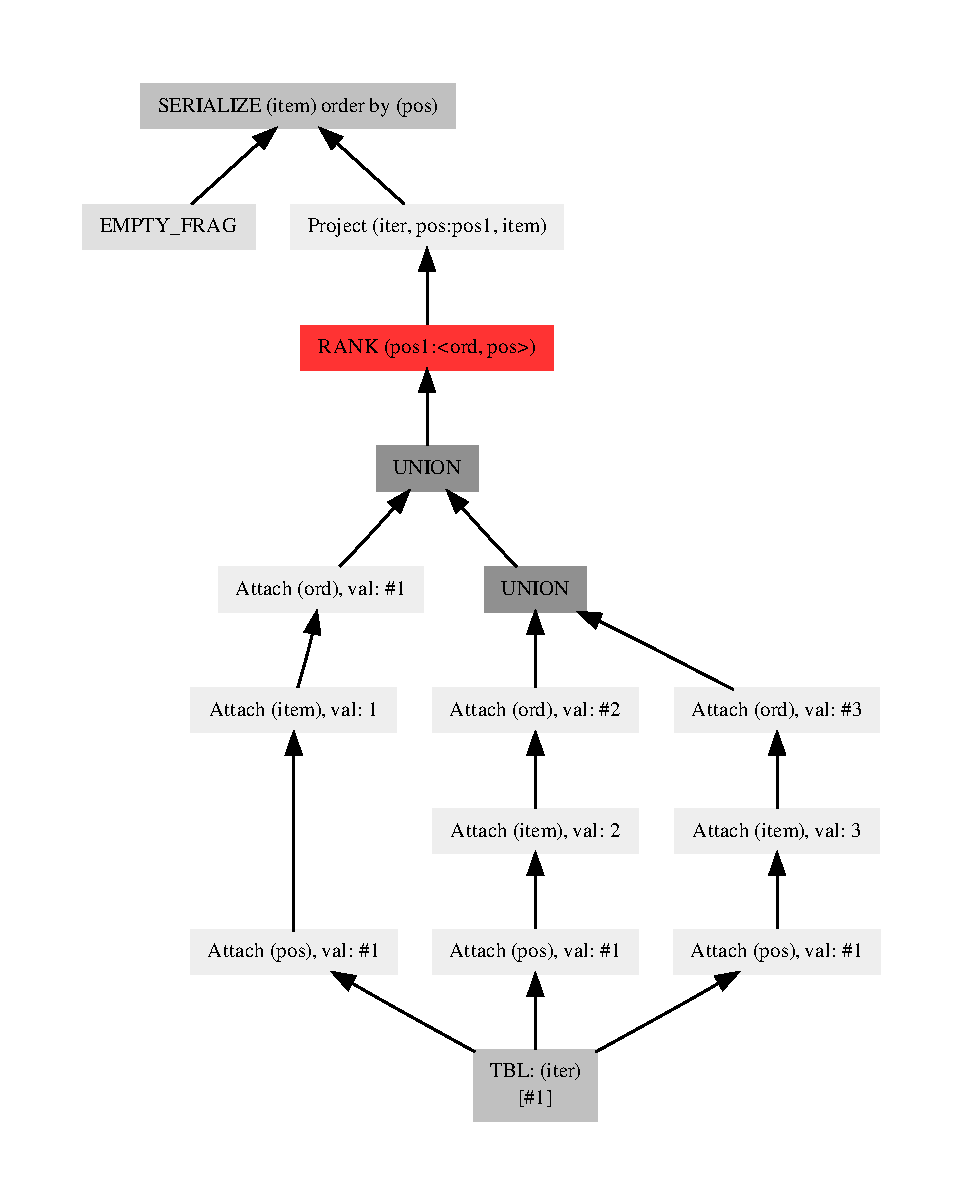
\includegraphics[width=0.4\textwidth]{img/graphs/td_impl_flwor_simple_pathfinder}
			\label{fig:result:comparison:simple_dag}
		}
		\quad
		\subfigure[Prototype implementation]{
		
			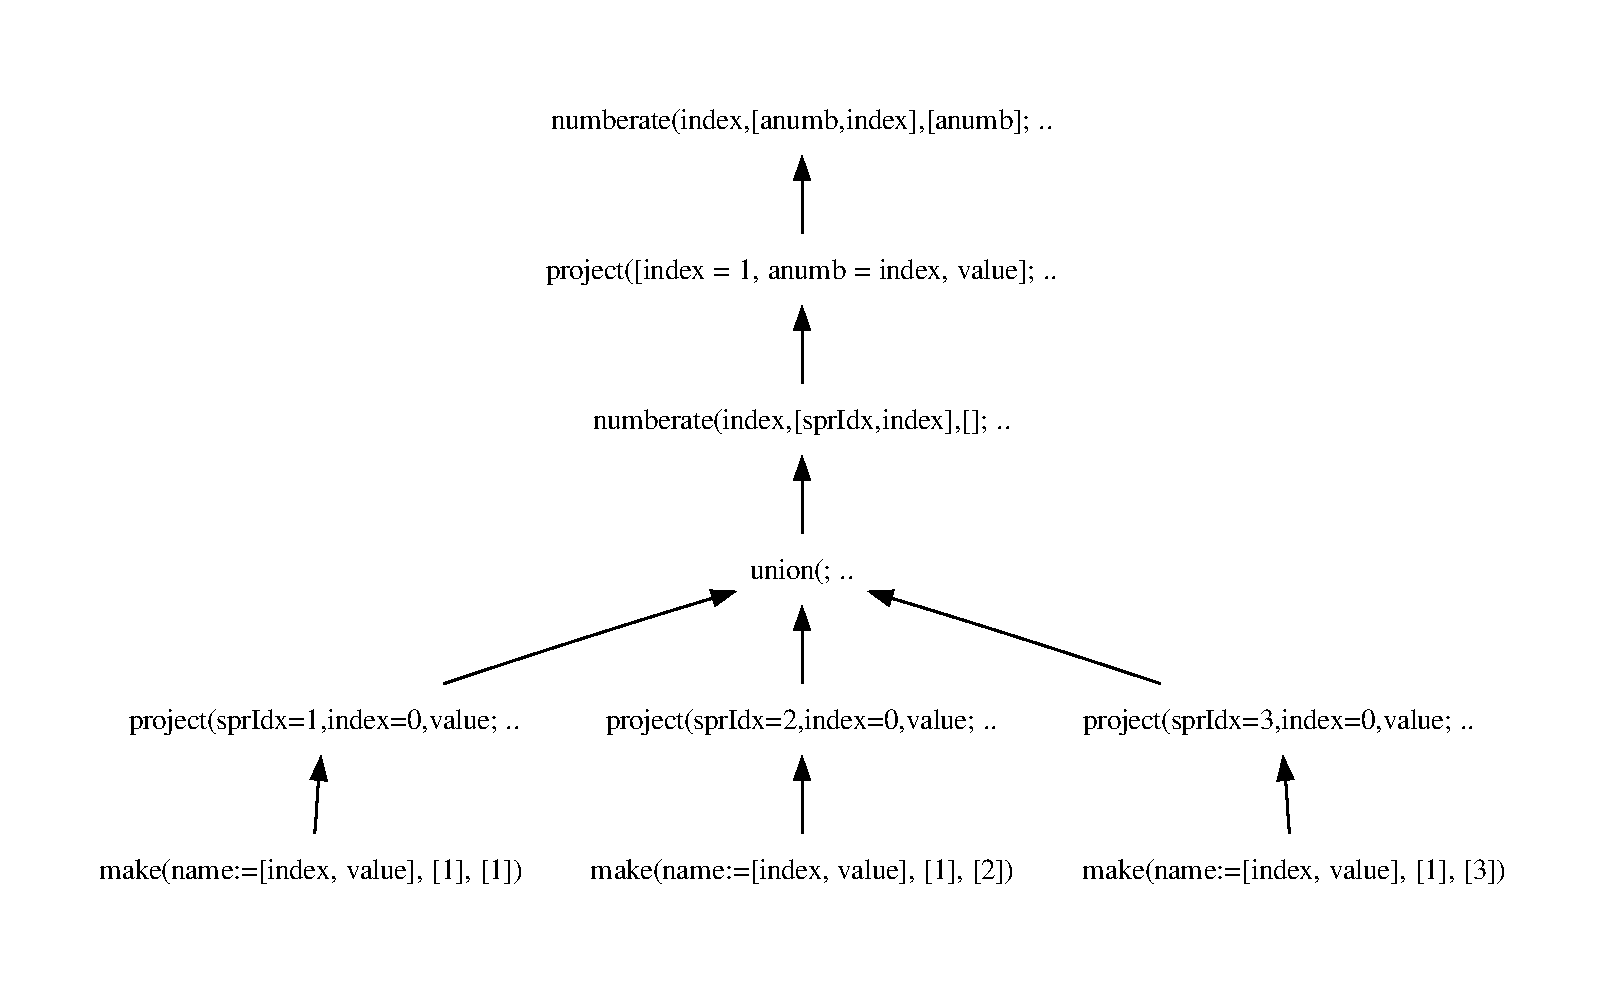
\includegraphics[width=0.6\textwidth]{img/graphs/td_impl_flwor_simple_xq_relalg}
			\label{fig:result:comparison:simple_pathfinder_dag}
		}
	}
	\caption{Comparison of DAGs for the trivial expression in section
	\ref{sect:results:algebra:generated:trivial_flwor}}
\end{figure}

\newpage
\begin{figure}[!h]
	\centering
	\mbox{
		\subfigure[MonetDB/Pathfinder]{		
			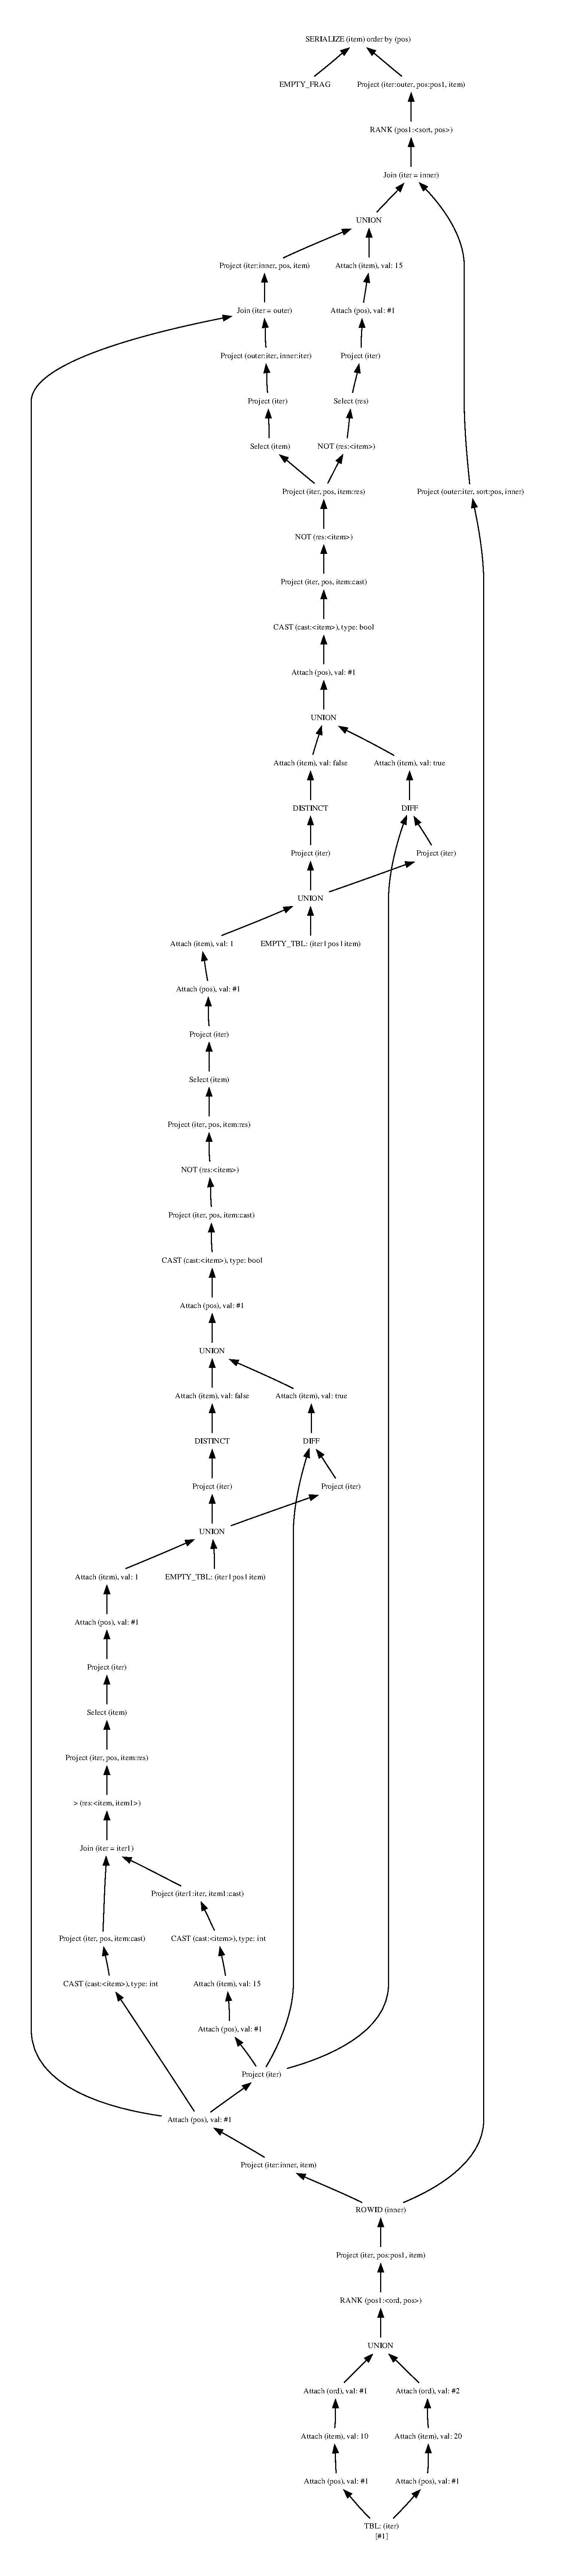
\includegraphics[width=0.3\textwidth]{img/graphs/td_impl_flwor_ifthenelse_pathfinder}
			\label{fig:result:comparison:conditional_dag}
		}
		\quad
		\subfigure[Prototype implementation]{
		
			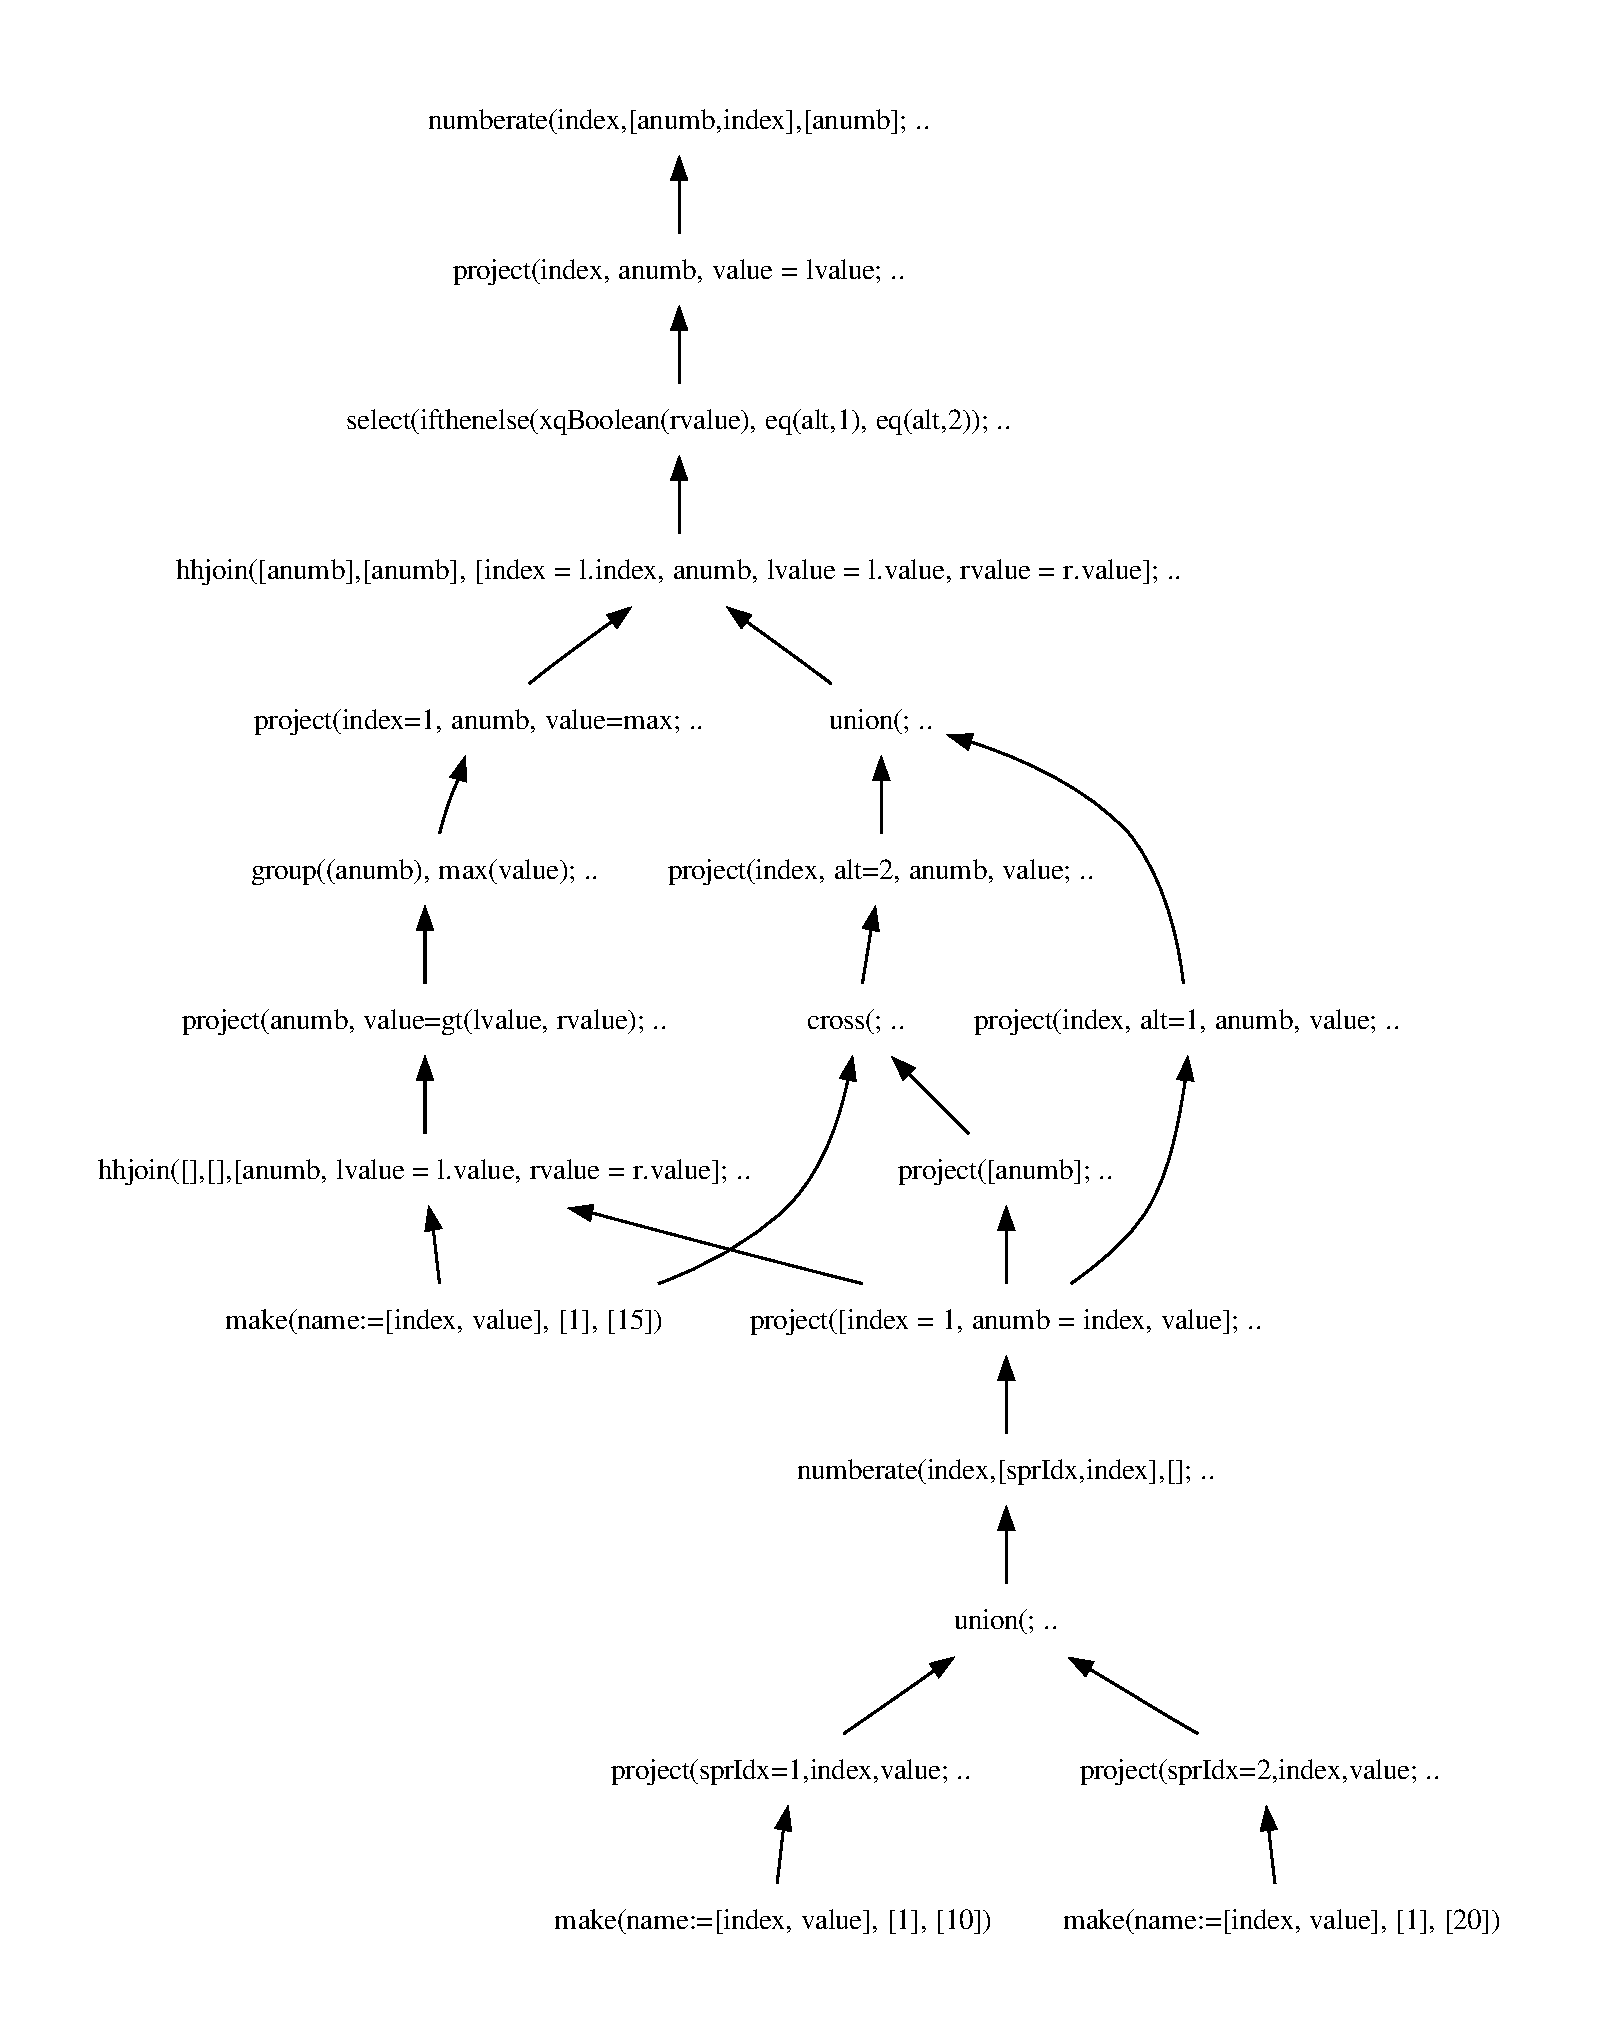
\includegraphics[width=0.7\textwidth]{img/graphs/td_impl_flwor_ifthenelse_xq_relalg_dag}
			\label{fig:result:comparison:conditional_pathfinder_dag}
		}
	}
	\caption{Comparison of DAGs for the conditional expression in section
	\ref{sect:results:algebra:generated:conditional_flwor}}
\end{figure}

\newpage
\begin{figure}[!h]
	\centering
	\mbox{
		\subfigure[MonetDB/Pathfinder]{		
			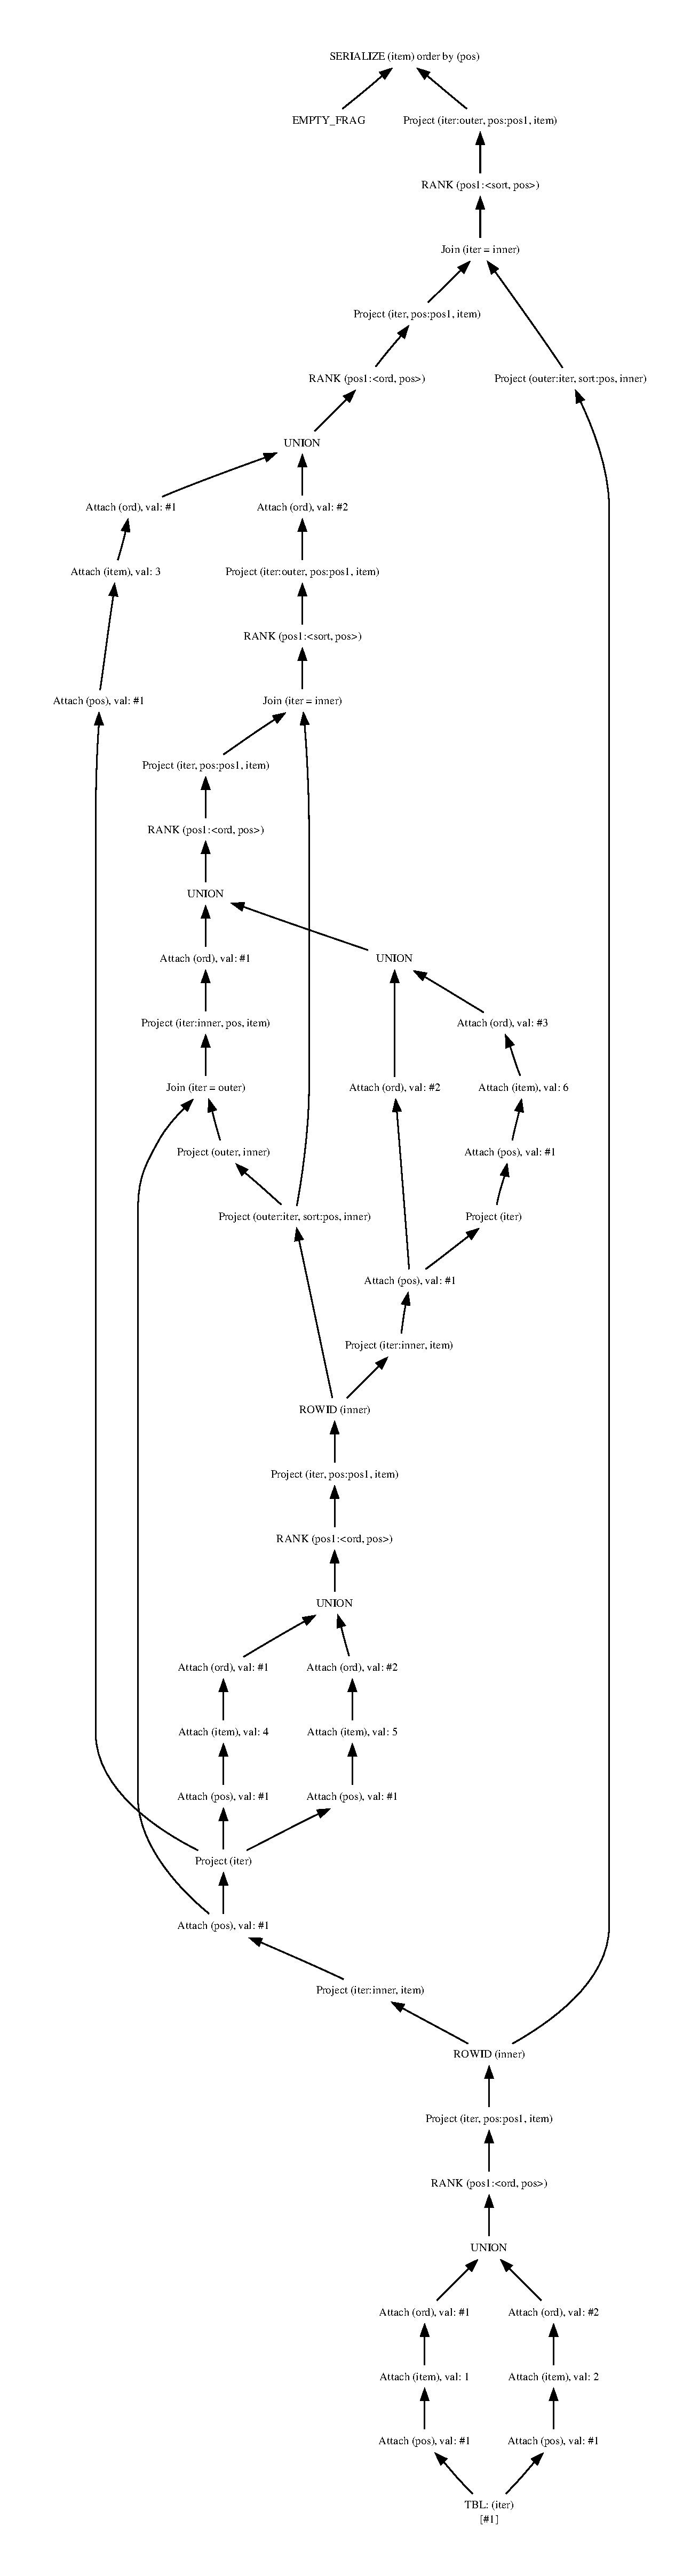
\includegraphics[width=0.37\textwidth]{img/graphs/td_impl_flwor_complex_pathfinder}
			\label{fig:result:comparison:complex_xqft_dag}
		}
		\quad
		\subfigure[Prototype implementation]{
		
			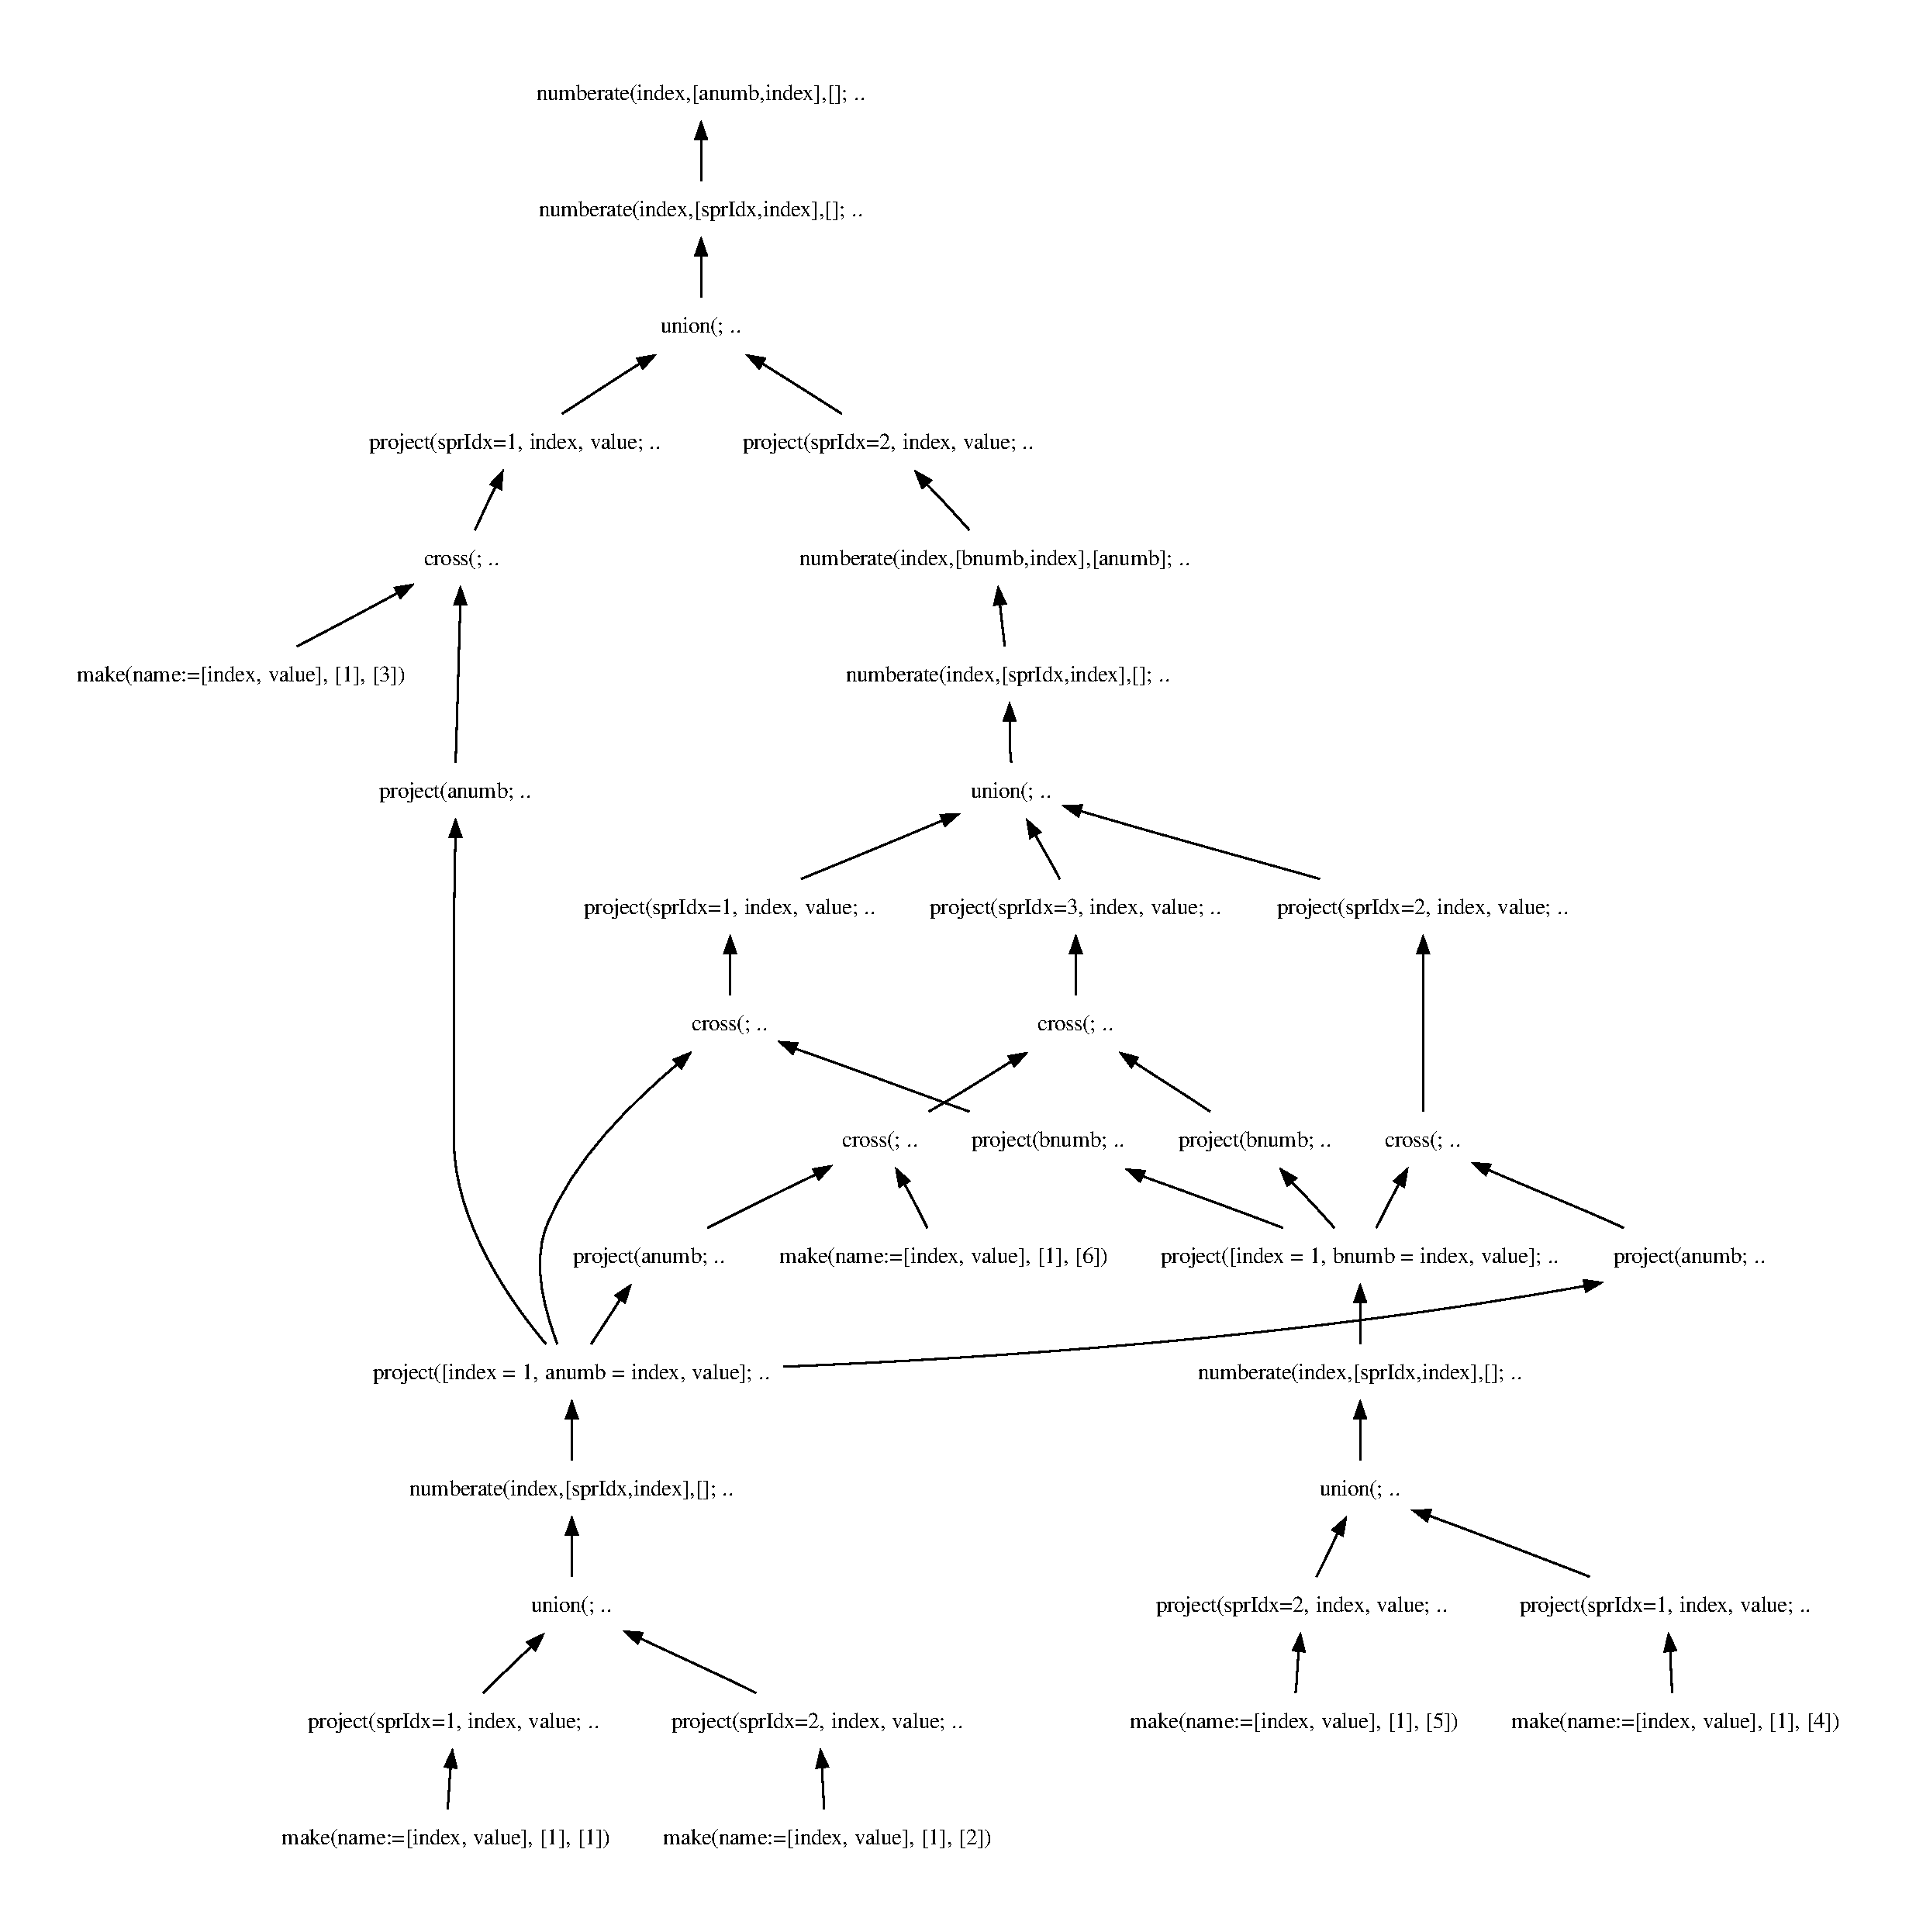
\includegraphics[width=0.6\textwidth]{img/graphs/td_impl_flwor_complex_xq_relalg_dag}
			\label{fig:result:comparison:complex_pathfinder_dag}
		}
	}
	\caption{Comparison of DAGs for the complex expression in section
	\ref{sect:results:algebra:generated:complex_flwor}}
\end{figure}

\newpage
\subsection{Complexity estimation and comparison}
Complexity estimation is performed as detailed in section
\ref{sect:method:complexity}. The complexity
comparison matrix is shown in table \ref{table:result:complexity_matrix}.

\begin{table}[!htp]
 \begin{tabular}{| c | c | c || c | c |}
  \hline
   & \multicolumn{2}{|c||}{\textbf{Pathfinder/MonetDB}}
   & \multicolumn{2}{|c|}{\textbf{Prototype implementation}} \\
   \hline
   & Tuples & Fields & Tuples & Fields \\  
   \hline
   Trivial & 16 & 16 & 15 & 18 \\  
   \hline
   Complex & 215 & 265 & 136 & 102 \\
   \hline
   Conditional & 94 & 50 & 31 & 44 \\  
   \hline
 \end{tabular}
\caption{Complexity comparison matrix}
\label{table:result:complexity_matrix}
\end{table}

\begin{figure}[!htp]
\begin{center}
  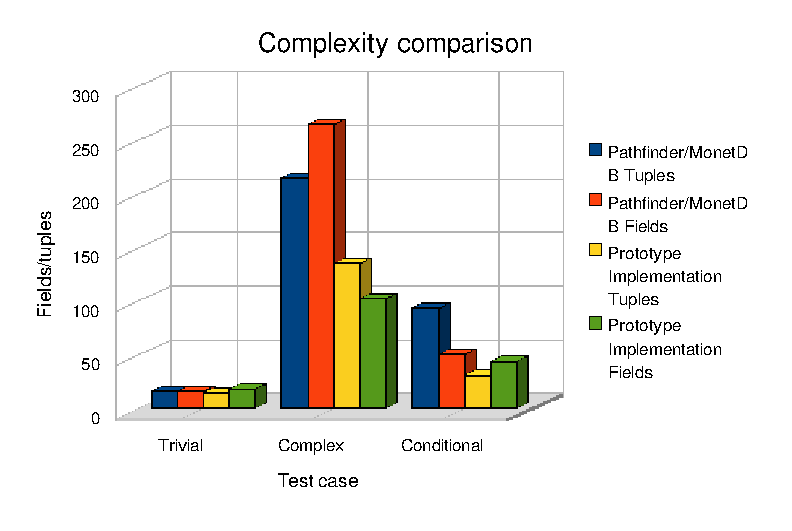
\includegraphics[width=1.0\textwidth]{diagrams/comparison_chart}
  \caption{Comparison chart}
  \label{fig:results:comparison:chart}
\end{center}
\end{figure}